\chapter{Theory of symmetric circulation}
\lastupdated{2024-12-13}{\chapterEightSymmCircOverleaf}

\begin{figure}[htpb]
	\centering
	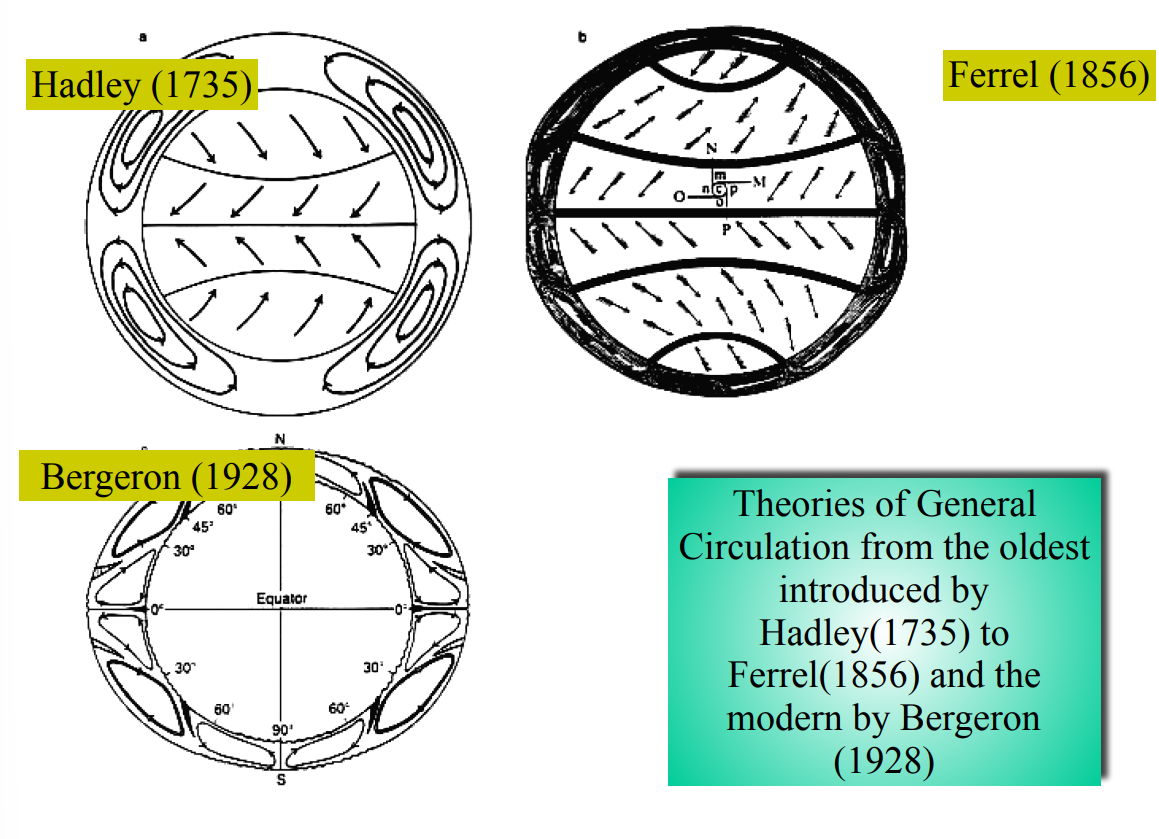
\includegraphics[width=0.35\linewidth]{uploads/Screenshot 2024-12-07 124123.png}
	\caption{History of the theories of the general circulation}

\end{figure}
In studying the general circulation of the atmosphere, a significant question arises: why does the \textbf{Hadley cell}, a key feature of the meridional circulation, extend only to about 30° latitude in each hemisphere? Why doesn’t it dominate the entire system, or extend further north or south? To answer these questions, we must delve into the dynamics of the Nonlinear Axially Symmetric Circulation\cite{I.Held1980} as explored by Isaac Held and others. Held analyzed a simplified atmospheric system by assuming symmetry around the Earth's axis. This eliminates longitudinal variations, allowing a focus on meridional (north-south) and vertical dynamics.\\


The general circulation of the atmosphere is composed of two major components, as described in the first chapter \ref{chapter1}:

\begin{enumerate}
	\item \textbf{Hadley Cell (Direct Circulation):} this thermally-driven circulation dominates the tropics and subtropics. Warm air rises near the Equator, flows poleward at high altitudes, sinks near 30° latitude, and returns equatorward near the surface as the trade winds.
	\item \textbf{Ferrel Cell (Indirect Circulation):} beyond 30° latitude, the circulation is opposite in direction, driven primarily by midlatitude dynamics rather than direct thermal forcing.
\end{enumerate}

Hadley theorized the existence of trade winds and a direct meridional circulation toward the poles, but his early model incorrectly predicted wind directions in midlatitudes. This error was resolved with the realization that the Earth’s rotation introduces Coriolis forces, altering the direction of winds and creating distinct circulation cells like the Ferrel cell.

Then why does the Hadley cell stop ad 30° latitude?

The Hadley cell limit is determined by the interplay of:
\begin{itemize}
	\item Coriolis Force: as air moves poleward, the Coriolis effect increases with latitude, deflecting the flow and limiting the extent of the Hadley circulation
	\item Angular momentum conservation: poleward moving air in the upper branch of Hadley cell accelerates as it conserves angular momentum, eventually leading to a breakdown into zonal (east-west) flow.
	\item Radiative forcing and thermal gradients: the temperature gradient between the Eq and the poles influences the location and strength of the Hadley cell.
\end{itemize}

To study the symmetric circulation, we simplify the governing equations by assuming:
\begin{enumerate}
	\item Axial Symmetry: the system is symmetric around the equator, eliminating longitudinal dependencies.
	\item Hydrostatic Balance: vertical pressure gradients balance gravity.
	\item Conservation of Mass (Continuity) divergence in the meridional plane (latitude-height) is zero.
	\item Prescribed Temperature Profile ($\Theta_E$): the system follows a latitudinally dependent potential temperature gradient.
\end{enumerate}
Using these assumptions, the Navier-Stokes equations reduce to a simpler form, looking at the time derivatives:
\[
	0 = -\nabla \cdot ({\overline{v}}{u}) + f v
	+ \frac{u v \tan \theta}{a}
	+ \frac{\partial}{\partial z} \left( \nu \frac{\partial u}{\partial z} \right)
\]

\[
	0 = -\nabla \cdot (v \overline{v}) - f u
	- \frac{u^2 \tan \theta}{a}
	+ \frac{\partial}{\partial z} \left( \nu \frac{\partial v}{\partial z} \right)
	- \frac{1}{a} \frac{\partial \Phi}{\partial \theta}
\]

\[
	0 = -\nabla \cdot ({\overline{v}} {\Theta})
	- \frac{1}{\tau} (\Theta - \Theta_E)
	+ \frac{\partial}{\partial z} \left( \nu \frac{\partial \Theta}{\partial z} \right)
\]

\[
	0 = -\nabla \cdot ({\overline{v}})
\]

\[
	\frac{\partial \Phi}{\partial z} = g \frac{\Theta}{\Theta_0}
\]
where $\overline{v}=(v,w)$ represents the velocity vector in the meridional plane, $$\nabla=\left[\frac{1}{a\cos\theta}\frac{\partial\cos\theta}{\partial\theta}, \frac{\partial}{\partial z}\right]$$ is the gradient operator.
$\Theta$ represents potential temperature.
$\Phi$ is the geopotential.
$a$ is the Earth's radius, $g$ is gravity, and $\nu$ represents viscosity.
These equations are written with the following approximations:
\begin{itemize}
	\item Steady, $(y,z)$, Boussinesq, dry, hemispheric
	\item Rigid lid at height H
	\item Forced by a linear "radiative" heating, chosen to be $$\frac{\Theta_E(\theta,z)}{\Theta_0}=1 - \frac{2}{3} \Delta_H P_2(\sin\theta) + \Delta_v \frac{z}{H} - \frac{1}{2}$$ where $\Theta_0$ is a global mean, $\Delta_H, \Delta_v$ are nondimensional constants that represents the fractional change in temperature from equator to pole and from the
	      top to the bottom, respectively. $P_2$ is the second Legendre polynomial.
	\item Vertical diffusion with constant diffusivity
	\item Zero stress boundary condition at the top and proportional to the surface wind at the bottom:
	      $$w=0\quad\frac{\partial u}{\partial z}=\frac{\partial v}{\partial z}=\frac{\partial\Theta}{\partial z}=0\quad\text{at}\quad z=H$$
	      $$w=0\quad\frac{\partial \Theta}{\partial z}=0,\quad v\frac{\partial u}{\partial z}=Cu,\quad v\frac{\partial v}{\partial z}=Cv\quad\text{at}\quad z=0$$
\end{itemize}

The zonal (east-west) wind $u$ is a function of latitude and height, while the meridional (north-south) wind $v$ is small or zero. The radiative forcing, structured by latitude and altitude, determines the thermal gradient from equator to pole, driving the circulation.


The equation of motion have a simple solution for the case in which there is no meridional flow ($v=0$). In this case also the vertical velocity is zero ($w=0$) and the temperature is in radiative equilibrium ($\Theta=\Theta_E$), the zonal wind satisfies:
\begin{equation}\label{13.3}
	\frac{\partial}{\partial z}\left(fu_E+\frac{u_E^2\tan\theta}{a}\right)=-\frac{g}{a\Theta_0}\frac{\partial\Theta_E}{\partial\theta}
\end{equation}
The vertical integration of the momentum equation and using the boundary condition implies that the zonal wind must be zero at the ground, so we can integrate \ref{13.3} and consider the solution obeying $u=0$ at $z=0$:
\begin{equation}\label{13.5}
	\frac{u_E}{\Omega_a}=\left[\left(1+\frac{2Rz}{H}\right)^{1/2}-1\right]\cos\theta\qquad R=\frac{gH\Delta_H}{\Omega^2a^2}
\end{equation}
The equations produce nonlinear solutions describing zonal flow. One notable solution shows a zonal westerly wind ($u>0$) increasing with height and latitude; the dynamics are controlled primary by rotation (Coriolis effect) and temperature gradients, encapsulated in a dimensionless parameter $R$, which determines the strength and extent of the circulation.\\


However, this solution has some difficulty. Considering the zonal momentum equation
\begin{equation}
	-\nabla\cdot(\vec{v}M)+\frac{\partial}{\partial z}\left(\nu\frac{\partial M}{\partial z}\right)=0
\end{equation}
where
$$M=u\times\theta=\Omega a^2\cos^2\theta+ua\cos\theta$$ is the angular momentum. We can ask ourselves where it can have a maximum. Hide\footnote{Hides theorem} showed that his maximum cannot be in the interior of the fluid. Assume in fact that such a maximum exist, then integration around a closed circuit sufficiently close to the maximum will get
$$\int\nabla\cdot(\vec{v}M)dl\approx M\int\nabla\cdot\vec{v}=0$$
for incompressibility, whereas the integral of the diffusion will not be zero. In practice, a maximum in the interior will be diffused away and the advection will not be capable to counteract. Instead it is possible to have a maximum close to the surface by vertically integrating the momentum equation where it is compensated by the stress boundary condition. The same condition will require that $u\leq 0$ at the surface. It follows that the angular momentum $M$ must be always smaller than its equatorial maximum ($\Omega a^2$) everywhere, yielding the condition
\begin{equation}\label{eq.umax}
	u<u_M=\frac{\Omega a\sin^2\theta}{\cos\theta}
\end{equation}
this is the solution that corresponds to the conservation of angular momentum. This means that the radiative solution $u_E$ cannot be valid until $u_E>u_M$. Using $\Delta_H=1/3$, $H=15$ km, we find $R\approx 0.2$ and therefore
$$\theta_h\leq27\text{°}$$
In this region the meridional velocity $v$ cannot be zero as required by the radiative balance.



Hence, we saw that if the angular momentum has a maximum inside the fluid, then we can make a contour around it, then integrate the angular momentum equation around it: the integral of the advection part will be zero, the integral of the diffusion will not. So there cannot be a maximum on the interior of the fluid, it will be on the surface, which will be compensated by the boundary condition. The solution $u_E$ cannot be valid everywhere but in the regions where it is greater than $u_M$ \ref{eq.umax} that corresponds to a certain latitude interval.

%REC
\subsubsection{Problems}
The extent of the Hadley circulation, which is currently confined to the tropics and subtropics, is sensitive to changes in the Earth's energy balance and rotation rate. \textbf{If climate change alters the equatorial temperature gradient or modifies energy conservation constraints, the Hadley cell could expand or contract, influencing global atmospheric patterns}.
The boundary of the Hadley cell, denoted as $\theta_h$, depends on key planetary and climatic parameters:

\begin{itemize}
	\item \textbf{Gravity ($g$)}: Stronger gravity limits the poleward extent of the Hadley cell, while weaker gravity allows it to expand further north or south.
	\item \textbf{Rotation Rate ($\Omega$)}: Faster rotation confines the Hadley cell closer to the equator, while slower rotation enables it to extend poleward.
	\item \textbf{Temperature Gradient ($\Delta T$)}: The difference in temperature between the equator and the poles drives the circulation, with larger gradients supporting more extensive cells.
\end{itemize}
On larger planets with slower rotation rates, the Hadley circulation tends to be smaller and less confined, as planetary rotation plays a weaker role in shaping the circulation.\\
[0.25cm]

We can be more precise on the estimate of $\theta_h$, i.e., the limit of the Hadley cell. Because a meridional flow must exist within a certain region close to the equator, let's assume that such circulation exists up to a certain latitude $\theta_h$. The poleward high altitude branch of the circulation conserves angular momentum so  $u(\theta,H)\approx u_M(\theta)$, but surface drag at the surface is sufficiently strong that $u(\theta,0)\approx 0$. Poleward of the limiting latitude $\theta_h$ the circulation is zero and in radiative equilibrium, $\Theta=\Theta_E$, $u=u_E$. We can evaluate the difference between the top ($z=H$) and the bottom ($z=0$) in \ref{13.3}:
\begin{equation}\label{13.10}
	f[u(H)-u(0)]+\frac{\tan\theta}{a}[u^2(H)-u^2(0)]=-\frac{gH}{a\Theta_0}\frac{\partial\{\Theta\}}{\partial\theta}
\end{equation}
where $\{\Theta\}$ denotes the vertical mean. Inserting
$$f=2\Omega\sin\theta\qquad u(H)=u_M=\frac{\Omega a}{\cos\theta}\sin^2\theta$$
and integrating from $0$ to $\theta$, we want to consider the difference between the vertical means:
\begin{equation}\label{13.12}
	\frac{\{\Theta(0)\}-\{\Theta(H)\}}{\Theta_0}\approx\frac{\Omega^2a^2\sin^4\theta}{2gH\cos^2\theta}\approx \frac{1}{2}\frac{\Omega^2a^2}{gH}\theta^4
\end{equation}
assuming small angles.

We also want to impose the continuity of potential temperature at latitude $\theta_h$:
\begin{equation}\label{13.13}
	\{\Theta(\theta_h)\}=\{\Theta_E(\theta_h)\}
\end{equation}

Combining \ref{13.12} with the \ref{13.13} integrated, that is:
$$\frac{\{\Theta_E\}}{\Theta_0}=\frac{\{\Theta_E(0)\}}{\Theta_0}-\Delta_H\theta^2$$
the solutions are
\begin{equation}
	\frac{\{\Theta(0)\}}{\Theta_0}=\frac{\{\Theta_E(0)\}}{\Theta_0}-\frac{5}{18}\Delta_HR\qquad \theta_h=\sqrt{\frac{5}{3}R}=\sqrt{\frac{5gH\Delta_H}{3\Omega^2}a^2}
\end{equation}
inserting numerical values we get
\begin{equation}\label{thetahadl}
	\theta_h\approx  26\text{°}
\end{equation}
This theory that is based on the conservation of angular momentum and of energy (via the conservation of potential temperature) then conclude that the extent of the Hadley cell is proportional to the square root of the equator-pole temperature gradient and to the square root of the height of the troposphere. It is instead inversely proportional to the rotation rate and the radius of the Earth, larger planets or faster planets will get smaller Hadley cells, whereas slower planets will result in larger Hadley cells.\\



We see how $\theta_h$ is a function of gravity, rotation of the planet, temperature change from equator to pole ($\rightarrow$ bigger planets have smaller Hadley circulation cell).
Changing rotational rate, how does that relation change?
\begin{figure}[htpb]
	\centering
	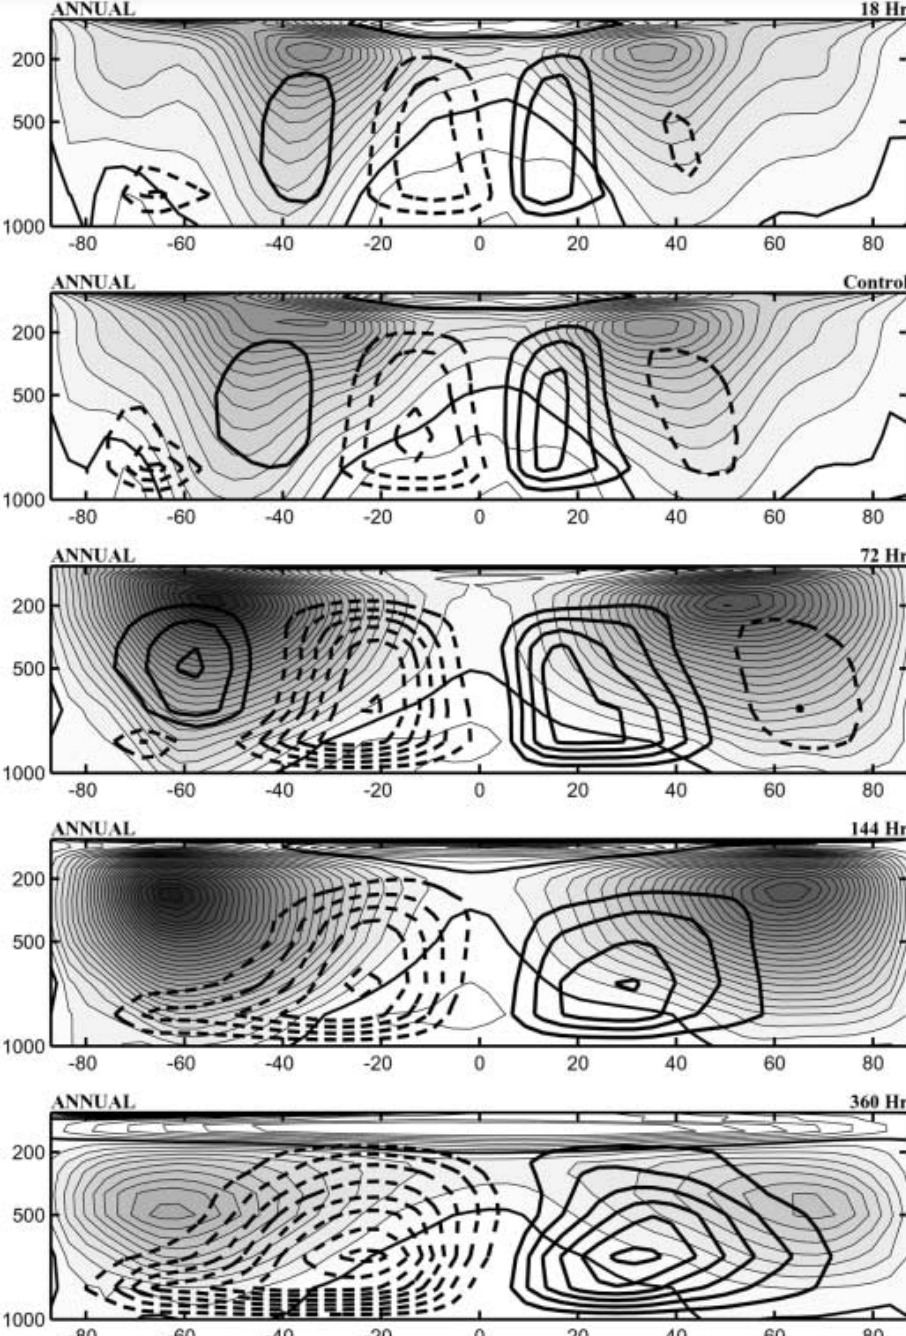
\includegraphics[width=0.35\linewidth]{uploads/cellsextent.png}
	\caption{decreasing Earth’s rotation rate on the Hadley circulation}
	\label{fig:decreasing rot rate}
\end{figure}
The figure (Figure \ref{fig:decreasing rot rate}) illustrates the impact of decreasing Earth's rotation rate on the Hadley circulation. Thick lines represent the streamfunction, indicating the direction of the flow:

\begin{enumerate}
	\item With Earth rotating at its current rate (24-hour day), the Hadley cell extends to about 30° latitude, with the Ferrel cell occupying the midlatitudes and storm tracks forming over these regions due to transient turbulence.
	\item If Earth's rotation slowed to a 72-hour day, the Hadley circulation would expand significantly, shifting its poleward boundary and the jet streams northward.
	\item With a rotation period of 360 hours (15 days), the Hadley cell would extend all the way to the poles, effectively eliminating the Ferrel cell.
\end{enumerate}
These simulations use a General Circulation Model (GCM), averaging results over time and incorporating conservation of momentum and energy.


The stability of the Hadley cell depends on how momentum is transported from the equator to the poles. In westerly momentum transport, the Hadley cell drives momentum poleward in the upper troposphere. Ferrel Cell and turbulence: the midlatitudes are dominated by transient eddies, which result from turbulent flow and instabilities.
\begin{figure}[htpb]
	\centering
	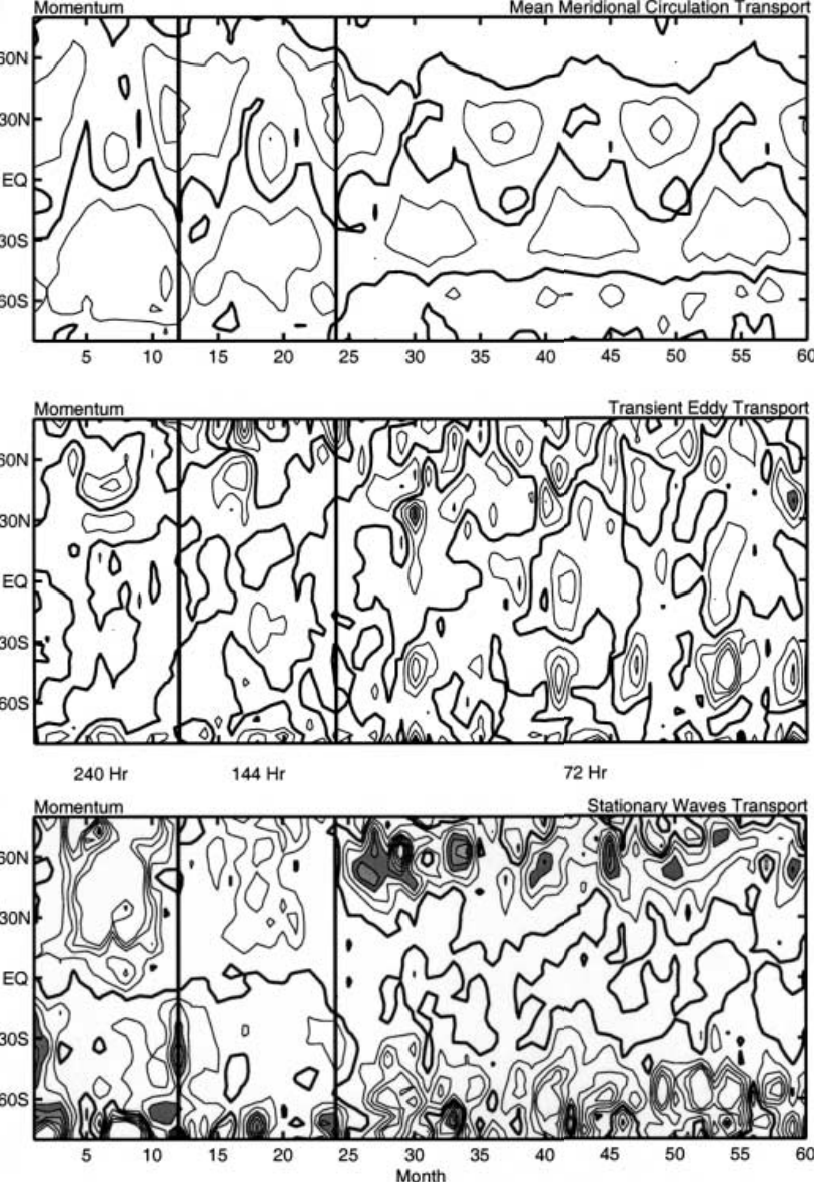
\includegraphics[width=0.35\linewidth]{uploads/stability of hadley cell.png}
	\caption{Stability of Hadley cell}
\end{figure}

As Earth's rotation slows (by approximately 1 hour every 100 million years due to tidal interactions), the momentum transport dynamics could change, potentially destabilizing current circulation patterns.


\paragraph{Precipitation and Storm Tracks}

Changes in the Hadley circulation's extent also affect precipitation patterns:

\begin{itemize}
	\item \textbf{Tropics}: Expanded Hadley circulation would shift tropical rainfall belts poleward.
	\item \textbf{Midlatitudes}: Storm tracks, driven by transient turbulence in the Ferrel cell, would move poleward, altering precipitation patterns in these regions.
\end{itemize}

\chapter{Tipping points}
\begin{figure}
	\centering
	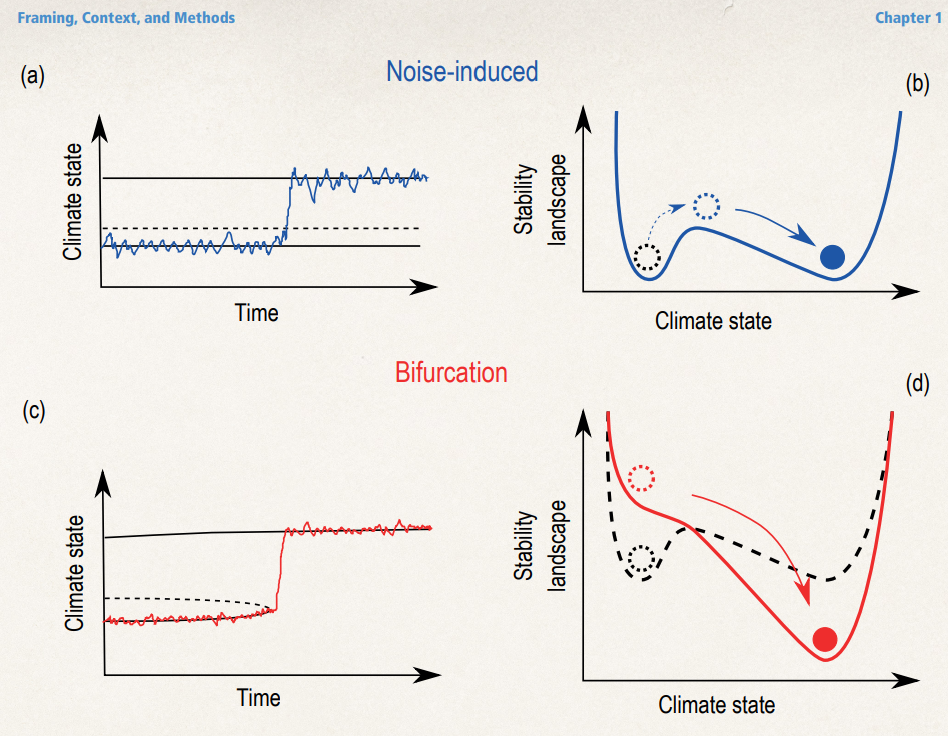
\includegraphics[width=0.45\linewidth]{uploads/tipping points.png}
	\caption{Illustration of two types of tipping points: noise-induced (a, b) and bifurcation (c, d). (a) and (c) are example time-series (coloured lines) through the tipping point, with solid-black lines indicating stable climate states (e.g., low or high rainfall) and dashed lines representing the boundary between stable states. (b) and (d) are stability landscapes, which provide an intuitive understanding of the different types of tipping point.}
	\label{fig:tippingpoints}
\end{figure}

An ‘abrupt change’ is defined in this report as a change that takes place substantially faster than the rate of change in the recent history of the affected component of a system. In some cases, abrupt change occurs because the system state actually becomes unstable, such that the subsequent rate of change is independent of the forcing. We refer to this class of abrupt change as a ‘tipping point’, defined as a critical threshold beyond which a system reorganizes, often abruptly and/or irreversibly. Tipping points are also referred to as planetary boundaries, they represent thresholds where rapid, often irreversible, changes occur in the climate system. These transitions typically involve fast dynamics combined with irreversibility, and they are often associated with bistable systems, which can exist in two distinct states (potential wells). Transitions between these states can be triggered either by noise-induced perturbations or by modifications of the underlying potential, often referred to as bifurcations.

In the figure \ref{fig:tippingpoints}, the ‘valleys’ represent different climate states the system can occupy, with ‘hilltops’ separating the stable states. The resilience of a climate state is implied by the depth of the valley. The current state of the system is represented by a ball. Both scenarios assume that the ball starts in the left-hand valley (dashed-black lines) and then through different mechanisms dependent on the type of tipping transitions to the right-hand valley (colored lines). Noise-induced tipping events (a, b), for instance drought events causing sudden dieback of the Amazon rainforest, develop from fluctuations within the system. The stability landscape in this scenario remains fixed and stationary. A series of perturbations in the same direction, or one large perturbation, are required to force the system over the hilltop and into the alternative stable state. Bifurcation tipping events (c, d), such as a collapse of the thermohaline circulation in the Atlantic Ocean under climate change, occur when a critical level in the forcing is reached. Here the stability landscape is subjected to a change in shape. Under gradual anthropogenic forcing the left-hand valley begins to shallow and eventually vanishes at the tipping point, forcing the system to transition to the right-hand valley. \\





The present rates of response of many aspects of the climate system are proportionate to the rate of recent temperature change, but some aspects may respond disproportionately. Some climate system components are slow to respond, such as the deep ocean overturning circulation and the ice sheets. It is virtually certain that irreversible, committed change is already underway for the slow-to-respond processes as they come into adjustment for past and present emissions. The paleoclimate record indicates that tipping elements exist in the climate system where processes undergo sudden shifts toward a different sensitivity to forcing, such as during a major deglaciation, where 1°C degree of temperature change might correspond to a large or small ice-sheet mass loss during different stages. For global climate indicators, evidence for abrupt change is limited, but deep ocean warming, acidification and sea level rise are committed to ongoing change for millennia after global surface temperatures initially stabilize and are irreversible on human time scales (very high confidence). At the regional scale, abrupt responses, tipping points and even reversals in the direction of change cannot be excluded (high confidence). Some regional abrupt changes and tipping points could have severe local impacts, such as unprecedented weather, extreme temperatures and increased frequency of droughts and forest fires. Models that exhibit such tipping points are characterized by abrupt changes once the threshold is crossed, and even a return to pre-threshold surface temperatures or to atmospheric carbon dioxide concentrations does not guarantee that the tipping elements return to their pre-threshold state. Monitoring and early warning systems are being put into place to observe tipping elements in the climate system.






\section{Examples of Climate System Tipping Points}

\begin{enumerate}
	\item \textbf{Gulf Stream and Heat Transport:} The Gulf Stream, a critical component of the Atlantic Meridional Overturning Circulation (AMOC), is unlikely to vanish entirely. However, its role in heat transport between the tropics and higher latitudes could be altered under changing climatic conditions. Such changes would have profound implications for regional and global climates.
	      \begin{figure}[htpb]
		      \centering
		      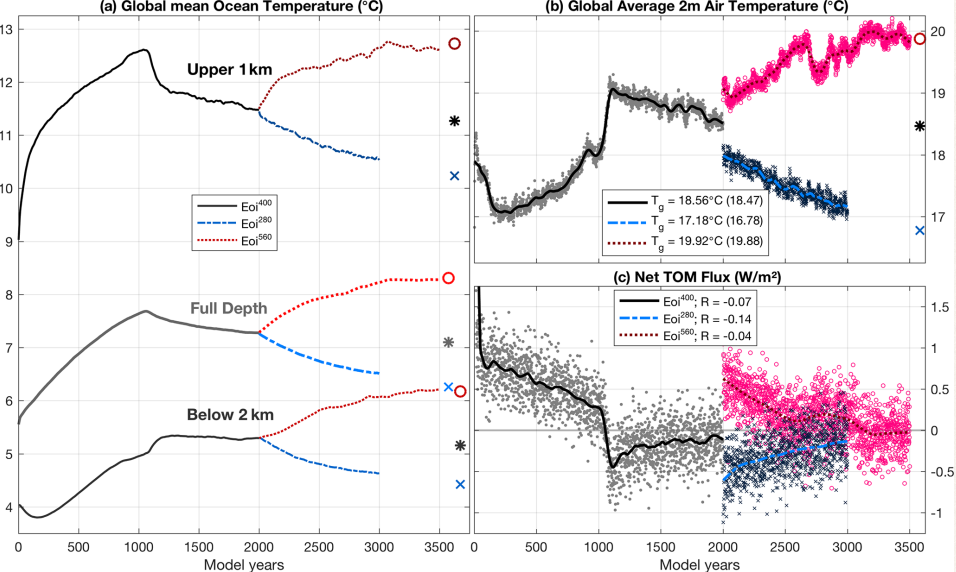
\includegraphics[width=0.5\linewidth]{uploads/temperature.png}
		      \caption{Time series of globally averaged temperatures for the entire length of our three different Pliocene simulations: Eoi400 (black), Eoi280 (blue), and Eoi560 (red). Shown are the (a) upper (dark), deep (medium), and full-depth (light) ocean temperature; (b) near-surface air temperature; and (c) globally averaged top-of-model (TOM) net radiative flux. Thick lines in (b) and (c) show the corresponding time series after applying a 100-year smoothing mask. The estimated equilibrium temperatures are indicated at the end in (a) and (b) using large markers and the same color convention. The globally averaged mean temperature (Tg in b) and net radiative flux (R in c) over the last 100 years are added in the legends (bracketed values for the estimated equilibrium). }
		      \label{fig:temperature}
	      \end{figure}
	\item \textbf{Sea Level Rise:}
	      \begin{itemize}
		      \item Thermal Expansion: as oceans warm, their volume increases due to thermal expansion, contributing significantly to sea level rise.
		      \item Melting Ice Sheets: ice melting currently contributes approximately 3 mm per year to global sea levels.
		      \item Solid Earth Adjustments: on longer timescales, the solid Earth is rebounding from the removal of massive ice sheets, a process known as isostatic adjustment.
		      \item Density Variations: sea level is also affected by changes in seawater density. For instance, increased salinity raises density, causing local sea levels to shrink.
	      \end{itemize}
	      \begin{figure}[htpb]
		      \centering
		      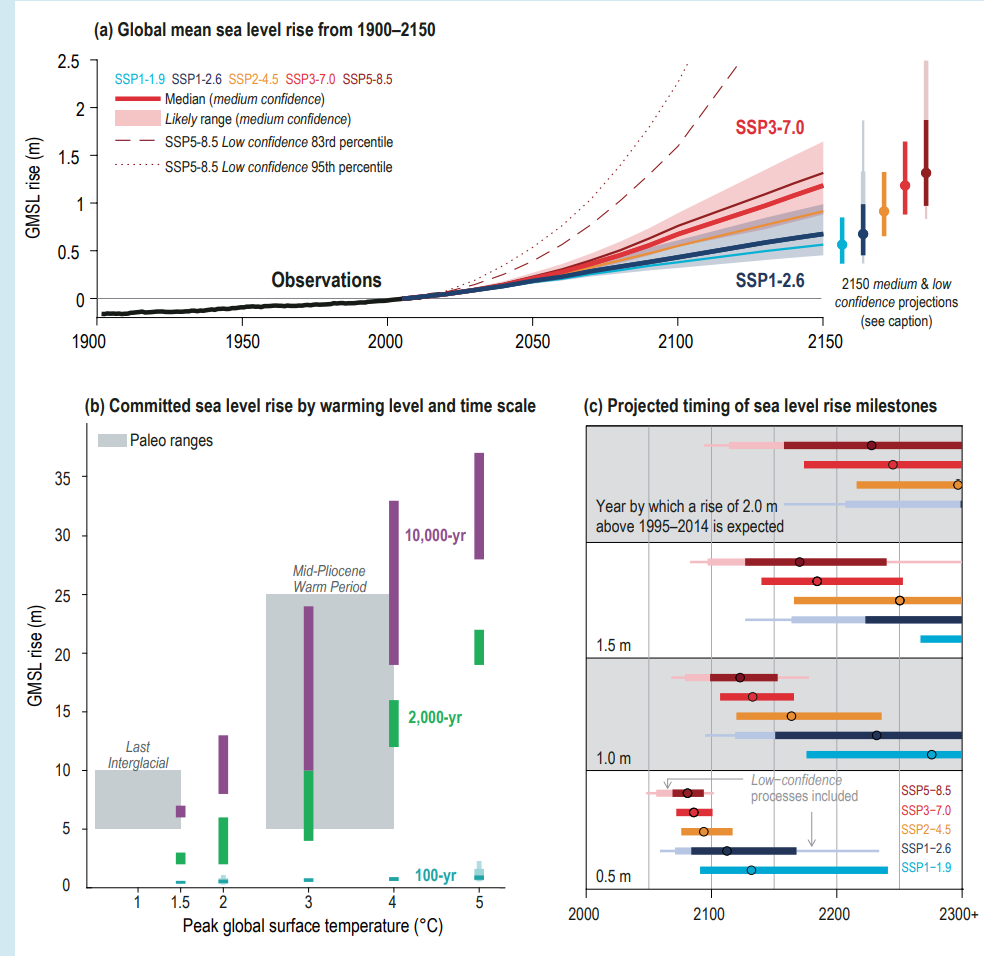
\includegraphics[width=0.5\linewidth]{uploads/sea level rise.png}
		      \caption{Sea level rise}
		      \label{fig:sea level rise}
	      \end{figure}







	\item \textbf{ENSO (El Niño–Southern Oscillation):} ENSO’s behavior is heavily influenced by the depth of the thermocline in the Pacific Ocean. If processes push the thermocline lower, there is the potential for a \textbf{permanent El Niño state}. This has been speculated as a possibility under higher CO$_2$ concentrations, reminiscent of conditions during the Pliocene epoch. However, current experiments are inconclusive regarding this outcome.
	      \begin{figure}[htpb]
		      \centering
		      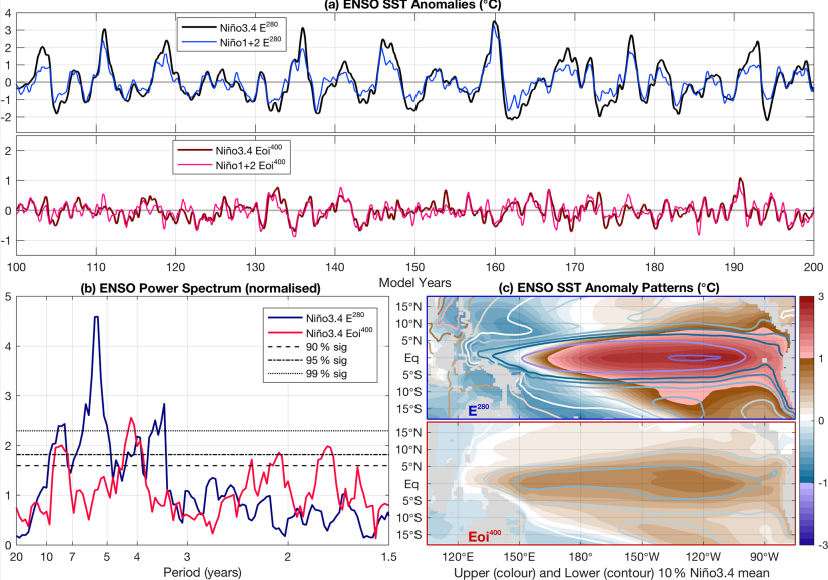
\includegraphics[width=0.5\linewidth]{uploads/ensotipping.png}
		      \caption{(a) ENSO time series for the E280 (blue) and Eoi400 (red) using monthly SST anomaly fields and a 5-month running mean. Note the different scaling. Temperature intervals are kept the same for visual comparison. (b) Multi-taper power spectrum, using 200 years of monthly data, including the 90 \%, 95 \%, and 99 \% confidence levels. (c) Corresponding ENSO SST patterns, taking the mean over the 10\% highest (shading) and 10\% lowest (contours) monthly Niño 3.4 index values. }
		      \label{fig:Ensotipping}
	      \end{figure}






	\item \textbf{Glaciations and Orbital Cycles}: major glaciations have occurred cyclically over the past 3 million years, with a periodicity of approximately 100,000 years. These glaciations are thought to be influenced by orbital forcing, as inferred from isotopic records. However, the exact causal mechanisms remain unclear. While carbon dioxide and glacial cycles covary, the time lag (approximately 10 years for CO$_2$ effects to manifest) complicates establishing causality.
\end{enumerate}
\begin{figure}[htpb]
	\centering
	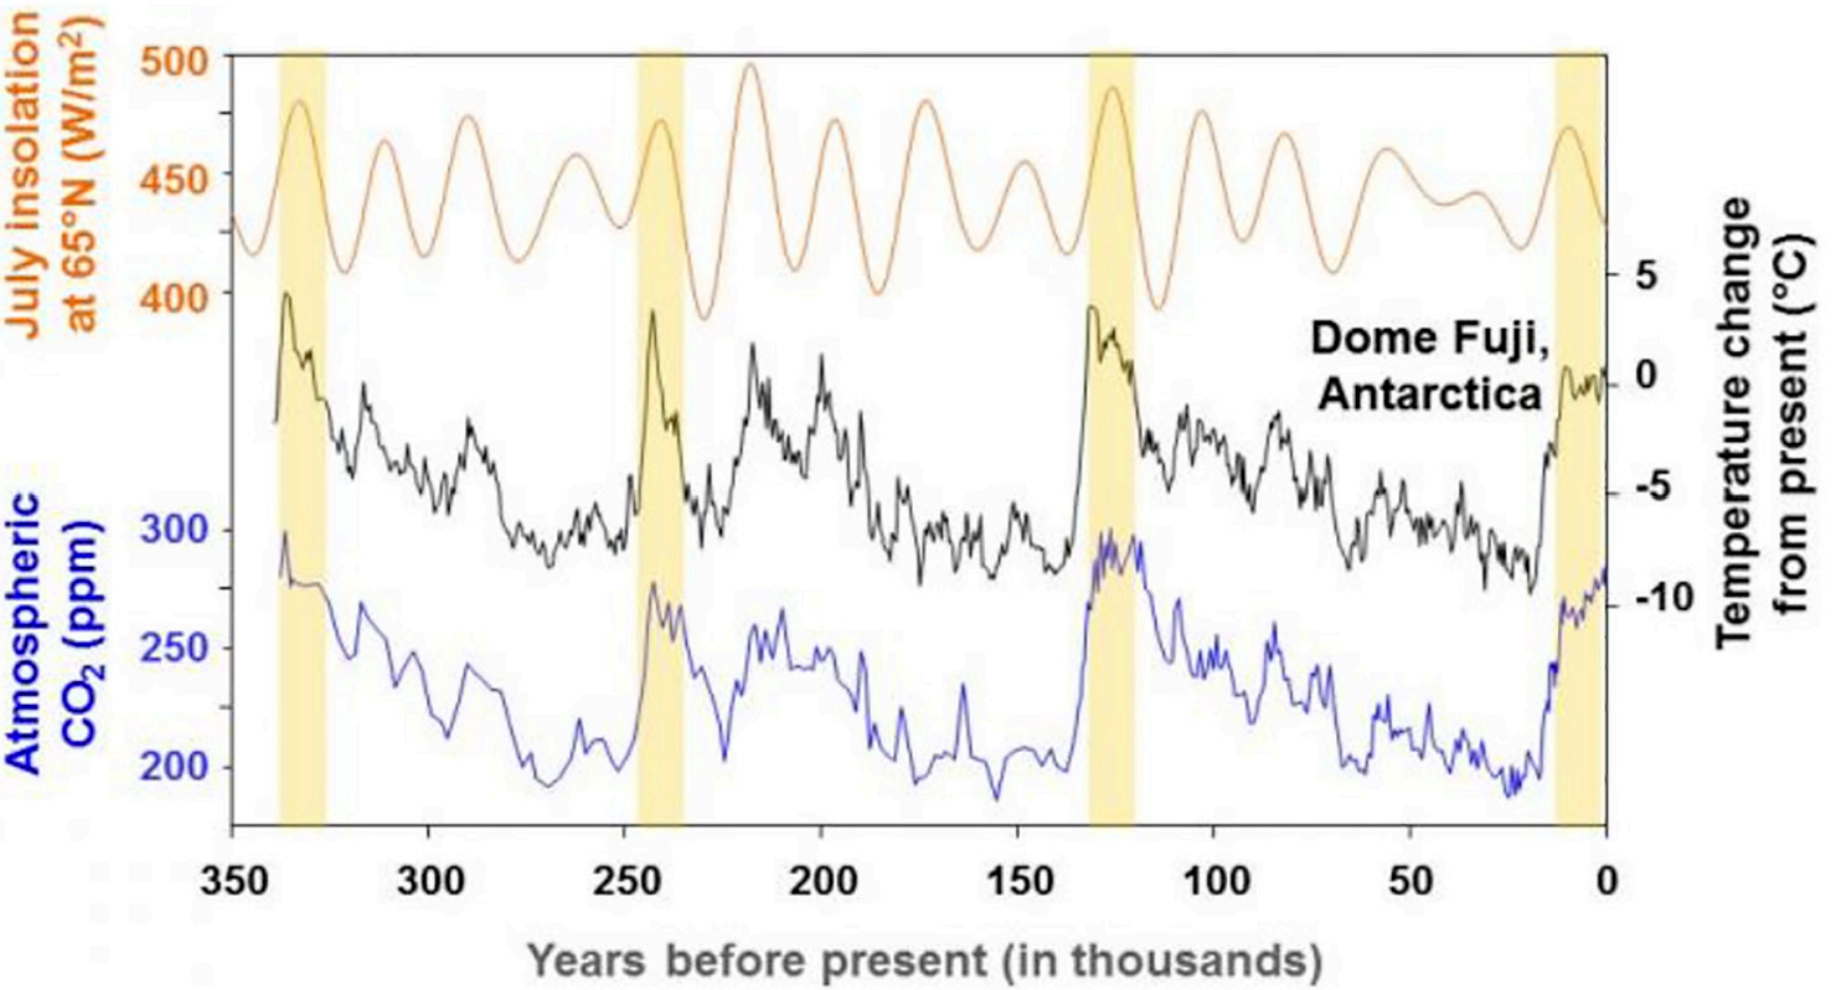
\includegraphics[width=0.5\linewidth]{uploads/glacial.png}
	\caption{Glacial cycles inferred from isotopic records}
	\label{fig:glacial cycles}
\end{figure}


\section{Climate impacts}

\begin{enumerate}
	\item \textbf{Regional Climate Impacts:} A collapse in systems like the AMOC or the establishment of a permanent El Niño state would drastically alter weather patterns, precipitation, and temperature distributions globally.
	\item \textbf{Sea Level Rise Feedbacks:} Dynamic processes such as shifting currents, salinity changes, and ice melt interact to exacerbate sea level changes, affecting coastal regions worldwide.
	\item \textbf{Climate Stabilization Challenges:} The path to stabilizing global temperatures involves achieving net-zero carbon emissions. Without this, many tipping points, once crossed, are irreversible.
\end{enumerate}

\paragraph{Modeling and Understanding Tipping Points}

Intermediate-complexity models such as \textbf{CLIMBER} are used to explore these phenomena. These models balance detailed physics with computational efficiency, allowing for longer timescales and broader parameter explorations.

\paragraph{Reversibility and Hysteresis}

Studies on hysteresis in climate systems investigate the potential for reversing climate change. While some tipping points (e.g., ice sheet loss) are deemed irreversible, others may exhibit pathways back to previous states under specific conditions. However, reducing east-west gradients in the Pacific through tipping-point dynamics, such as those involving ENSO, remains a critical area of ongoing research.
We cannot stabilize the temperature without going to \textbf{net 0} emissions.\\



xx babies

\chapter{Are General Circulation models obsolete?}